\label{sec:fluid}
In order to understand the motivations for, as well as the limitations and the behaviour of, the experiment we need to know about a few key concepts in fluid mechanics.

\subsection{Reynolds number}
The Reynolds number ($\operatorname{Re}$) is a dimensionless number describing the ratio of the strength of inertial forces to the strength viscous forces in a flow. Roughly speaking one can think of viscous forces as acting to keep adjacent fluid elements moving in the same direction whereas inertial forces act to prevent any change in the motion of a fluid element. For a flow it is defined as \cite{introfluid}

\begin{equation}\label{eq:reynolds}
\operatorname{Re} = \frac{U W \rho}{\mu}
\end{equation}
where $U$ is the characteristic velocity of the flow, $W$ is its characteristic length scale, $\rho$ is the density of the fluid, and $\mu$ is its dynamic viscosity. The Reynolds number is used to characterize the regime of the flow. There are two primary regimes
\begin{enumerate}
\item Laminar regime, where viscous forces dominate over inertial forces.
\item Turbulent regime where inertial forces dominate.
\end{enumerate}

\noindent A simple visual characterization of the flow types can be seen in Figure \ref{fig:laminar_flow}. 

Flow with $\operatorname{Re}\ll 1$ is referred to as \emph{Stokes flow}. In this regime we can ignore inertial forces completely. The flow is guaranteed to be laminar, and it is also time reversible. This means any dynamics of the fluid are retraced when the flow is reversed, as if time was reversed. ~\cite{introfluid3}
 
Particles in Stokes flow are also time reversible if they have a particle Reynolds number $\Re << 1$. The particle Reynolds number is defined as \cite{JonasLic}

\begin{equation}\label{eq:reynoldsparticle}
\operatorname{Re_p} = \frac{u_p L \rho}{\mu}
\end{equation}

where $u_p$ is the typical flow speed relative to the particle surface, $L$ is the characteristic size of the particle, $\rho$ is the density of the fluid and $\mu$ is the dynamic viscosity of the fluid. 

\begin{figure}[H]
\centering
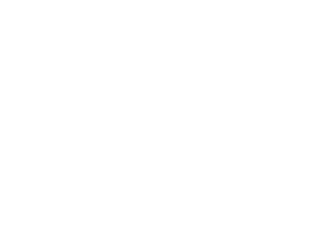
\includegraphics[width=0.6\textwidth]{figures/theory/laminarFlow.pdf}
\caption{This shows the principal difference between laminar and turbulent flow.}
\label{fig:laminar_flow}
\end{figure}

\subsection{Stokes drag and Stokes' law}
For $\operatorname{Re} = 0$ the drag force $F_D$ exerted by a fluid on a spherical particle is found using Stokes's law \cite{introfluid2}

\begin{equation}\label{eq:stokes_law}
F_D = 6\pi \mu R v.
\end{equation}

\noindent Here $v$ is the velocity of the sphere relative to the fluid, $\mu$ is the dynamic viscosity, and $R$ is the radius of the sphere. This can be used to find the terminal velocity of a sphere sinking in a liquid by equating the gravitational force $F_G$ acting on the sphere with the drag force from eq \ref{eq:stokes_law}. $F_G$ is calculated as

\begin{equation}
F_G = \Delta \rho g \frac{4\pi R^3}{3},
\end{equation}

\noindent where $\Delta \rho$ is the difference in density between the fluid and the sphere and $g$ is the specific gravity. We find that the terminal velocity of a sinking (or floating) sphere is

\begin{equation}\label{eq:fallingSphere}
v_s = \frac{2}{9} \frac{\Delta \rho}{\mu} g R^2.
\end{equation}

\noindent This is not immediately applicable to cylindrical particles but serves as a first order approximation.